\documentclass{article}

\usepackage[utf8]{inputenc}
\usepackage[russian]{babel}
\usepackage{graphicx}
\graphicspath{{pictures/}}
\DeclareGraphicsExtensions{.pdf,.png,.jpg}
\usepackage[unicode, pdftex]{hyperref}
\usepackage{csvsimple}

\begin{document}

\begin{titlepage}
  \thispagestyle{empty}
  \centerline {Санкт-Петербургский политехнический университет}
  \centerline { им. Петра Великого}
  \centerline { }
  \centerline {Институт прикладной математики и механики} 
  \centerline {Кафедра "Прикладная математика"}
  \vfill
  \centerline{\textbf{Отчёт}}
  \centerline{\textbf{по лабораторной работе №3}}
  \centerline{\textbf{по дисциплине}}
  \centerline{\textbf{"Математическая статистика"}}
  \vfill
  \hfill
  \begin{minipage}{0.45\textwidth}
  Выполнил студент:\\
  Дроздова Дарья Александровна\\
  группа: 3630102/80401 \\
  \\
  Проверил:\\
  к.ф.-м.н., доцент \\
  Баженов Александр Николаевич
  \end{minipage}
  \vfill
  \centerline {Санкт-Петербург}   
  \centerline {2021 г.}  
\end{titlepage}

\newpage
\setcounter{page}{2}
\tableofcontents

\newpage
\listoftables

\newpage
\listoffigures

\newpage
\section{Постановка задачи}
Для 5 распределений:
  \begin{itemize}
    \item Нормальное распределение: $N(x,0,1)$
    \item Распределение Коши: $C(x,0,1)$
    \item Распределение Лапласа: $L(x,0,\sqrt{2})$
    \item Распределение Пуассона: $P(k,10)$
    \item Равномерное распределение: $U(x,-\sqrt{3}, \sqrt{3})$
  \end{itemize}
Сгенерировать выборки мощностью 20 и 100 элементов. Построить для них боксплот Тьюки. Для каждого распределения определить долю выбросов эксперементально и сравнить с теоретическим результатом.

\newpage
\section{Теория}
\subsection{Боксплот Тьюки}
Боксплот Тьюки - график, использующийся в описательной статистике, компактно изображающий одномерное распределение вероятностей.
\begin{figure}[h]
\center{\includegraphics[scale=0.7]{boxplot}}
\caption{Боксплот Тьюки}
\end{figure} \\
Граница ящика - первый и третий квартили, линия в середине - медиана. Концы усов - края статистически значимой выборки. Длина "усов":
\begin{equation}
X_1 = Q_1 - \frac{3}{2}(Q_3 - Q_1)
\label{eq:1}
\end{equation}
\begin{equation}
X_2 = Q_3 + \frac{3}{2}(Q_3 - Q_1)
\label{eq:2}
\end{equation}
где $X_1$ - нижняя граница уса, $X_2$ - верхняя граница уса, $Q_1$ - первый квартиль, $Q_3$ - третий квартиль. \\
Выбросы изображаются на графике в виде кружочков.
\subsection{Классификация распределений}
Распределения принято классифицировать по характеру функций распределения. \\
Классификация распределений:
\begin{itemize}
  \item Дискретные распределения
  \item Решётчатые распределения
  \item Непрерывные распределения
  \item Сингулярные распределения
\end{itemize}
В данной лабораторной работе рассматриваются непрерывные и дискретные распределения. \\
Непрерывные распределения:
\begin{itemize}
    \item Нормальное распределение: $N(x,0,1)$
    \item Распределение Коши: $C(x,0,1)$
    \item Распределение Лапласа: $L(x,0,\sqrt{2})$
    \item Равномерное распределение: $U(x,-\sqrt{3}, \sqrt{3})$
\end{itemize}
Дискретные распределения:
\begin{itemize}
    \item Распределение Пуассона: $P(k,10)$
  \end{itemize}
\subsection{Выбросы}
Если вычислить теоретическую нижнюю и верхнюю границы уса $X_1^T, X_2^T$ по формулам (\ref{eq:1}), (\ref{eq:2}), то можно определить величины выбросов $x$, которые определяются по формуле:
\begin{equation}
  \left[\ 
  \begin{array}{rcl}
  x < X_1^T \\
  x > X_2^T
  \end{array}\right.
  \label{eq:3}
\end{equation}
Теоретическая вероятность выбросов для непрерывных распределений:
\begin{equation}
P_H^T = P(x < X_1^T) + P(x > X_2^T) = F(X_1^T) + (1 - F(X_2^T)
\label{eq:4}
\end{equation}
где $F(X)=P(x \le X)$ - функция распределения. \\
Теоретическая вероятность выбросов для дискретных распределений:
\begin{equation}
P_H^T = P(x < X_1^T) + P(x > X_2^T) = (F(X_1^T) - P(x = X_1^T) + (1 - F(X_2^T))
\label{eq:5}
\end{equation}
где $F(X)=P(x \le X)$ - функция распределения.

\newpage
\section{Реализация}
Лабораторная работа выполнена на языке программирования Python в среде разработки PyCharm с использованием библиотек: numpy, skipy для построения выборок и функции распределения вероятности. А также использовалась библиотека pyplot для построения боксплота.
\\
\\
Код программы расположен в репозитории GitHub по ссылке: \url{https://github.com/Drozdova-Daria/Math_Stat_Lab3}

\newpage
\section{Результаты}
\subsection{Боксплот Тьюки}
\subsubsection{Нормальное распределение}
\begin{figure}[h]
\center{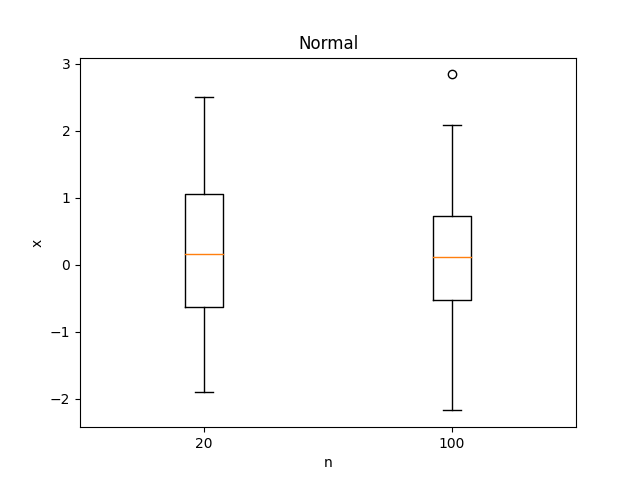
\includegraphics[scale=0.5]{Normal}}
\caption{Боксплот Тьюки для нормального распределения}
\end{figure}
\subsubsection{Распределение Коши}
\begin{figure}[h]
\center{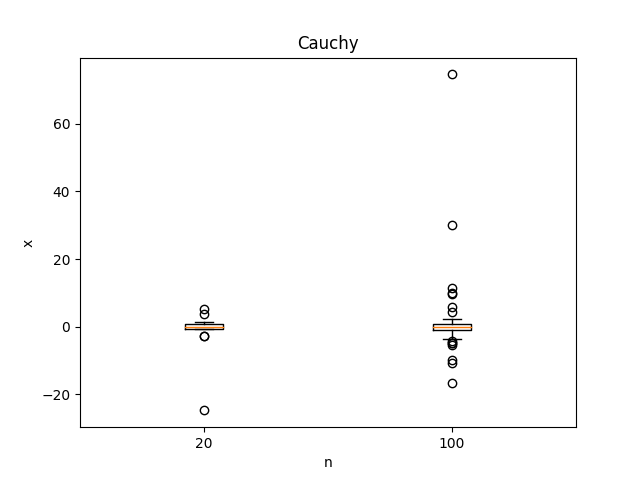
\includegraphics[scale=0.5]{Cauchy}}
\caption{Боксплот Тьюки для распределения Коши}
\end{figure}
\subsubsection{Распределение Лапласа}
\begin{figure}[h]
\center{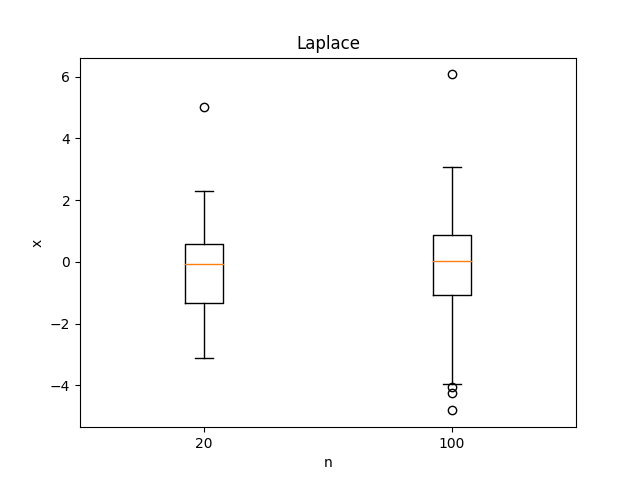
\includegraphics[scale=0.5]{Laplace}}
\caption{Боксплот Тьюки для распределения Лапласа}
\end{figure}
\subsubsection{Распределение Пуассона}
\begin{figure}[h]
\center{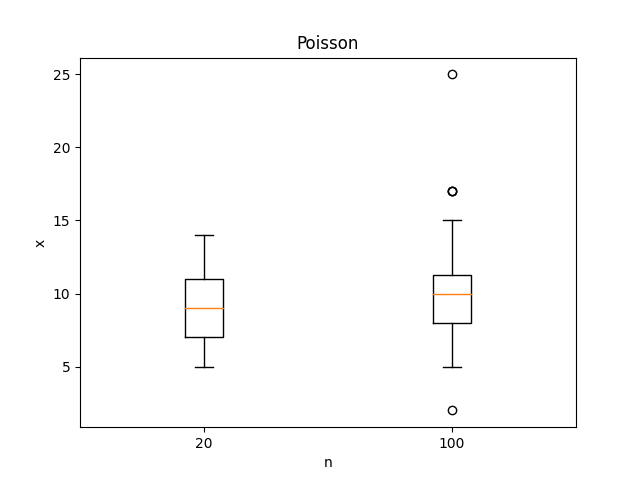
\includegraphics[scale=0.5]{Poisson}}
\caption{Боксплот Тьюки для распределения Пуассона}
\end{figure}
\; \\ \; \\ \;
\subsubsection{Равномерное распределение}
\begin{figure}[h]
\center{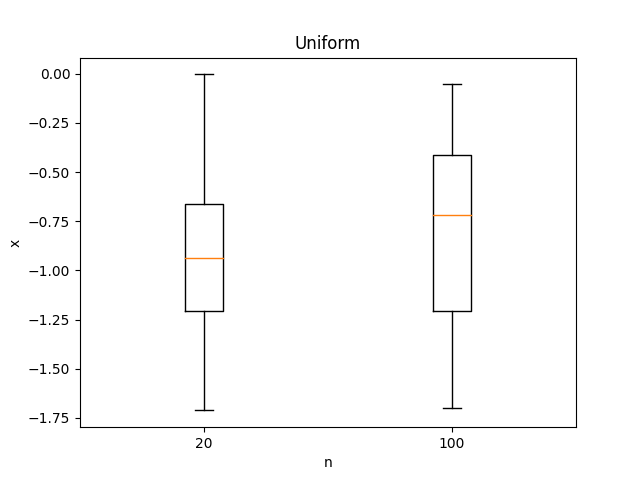
\includegraphics[scale=0.5]{Uniform}}
\caption{Боксплот Тьюки для равномерного распределения}
\end{figure}
\subsection{Фактическая доля выбросов}
\begin{table}[hb]
\begin{center}
\begin{tabular}{|c|c|c|}
\hline 
Вид распределения & Мощность выборки & Доля выбросов \\ 
\hline 
Нормальное & 20 & 0.023 \\ 
\hline 
Нормальное & 100 & 0.009 \\ 
\hline 
Коши & 20 & 0.149 \\ 
\hline 
Коши & 100 & 0.154 \\ 
\hline 
Лапласа & 20 & 0.075 \\ 
\hline 
Лапласа & 100 & 0.065 \\ 
\hline 
Пуассона & 20 & 0.025 \\ 
\hline 
Пуассона & 100 & 0.011 \\ 
\hline 
Равномерное & 20 & 0.003 \\ 
\hline 
Равномерное & 100 & 0.0 \\ 
\hline 
\end{tabular} 
\caption{Фактическая доля выбросов}
\end{center}
\end{table}
\; \\ \; \\ \; \\ \; \\ \; 
\subsection{Теоретическая вероятность выбросов}
\begin{table} [hb]
\begin{center}
\begin{tabular}{|c|c|c|c|c|c|c|}
\hline 
Вид распределения & Мощность выборки & $Q_1^T$ & $Q_3^T$ & $X_1^T$ (\ref{eq:1})& $X_2^T$ (\ref{eq:2})& $P_B^T$ (\ref{eq:4}),(\ref{eq:5}) \\ 
\hline 
Нормальное & 20 & -1.2191 & 0.1801 & -3.3179 & 2.2788 & 0.0118 \\ 
\hline 
Нормальное & 100 & -0.5037 & 0.8335 & -2.5094 & 2.8392 & 0.0083 \\ 
\hline 
Коши & 20 & -0.9413 & 0.2128 & -2.6724 & 1.944 & 0.2652 \\ 
\hline 
Коши & 100 & -0.8962 & 0.9409 & -3.6519 & 3.6966 & 0.1692 \\ 
\hline 
Лапласа & 20 & -1.7987 & 1.2538 & -6.3775 & 5.8326 & 0.0136 \\ 
\hline 
Лапласа & 100 & -0.7183 & 1.0526 & -3.3745 & 3.7088 & 0.0823 \\ 
\hline 
Пуассона & 20 & 8.0 & 11.25 & 3.125 & 16.125 & 0.0374 \\ 
\hline 
Пуассона & 100 & 8.0 & 11.0 & 3.5 & 15.5 & 0.0591 \\ 
\hline 
Равномерное & 20 & -1.2679 & -0.6699 & -2.1649 & 0.2271 & 0.0 \\ 
\hline 
Равномерное & 100 & -1.3477 & -0.4264 & -2.7298 & 0.9556 & 0.0 \\ 
\hline 
\end{tabular} 
\caption{Теоретическая вероятность выбросов}
\end{center}
\end{table}

\newpage
\section{Обсуждение}
Боксплот Тьюки позволяет получить наглядную оценку важных характеристик распределения. \\
Исходя из таблиц теоретической и фактической доли выбросов можно сделать следующие выводы. Чем больше мощность выборки тем ближе фактическая доля выбросов к теоретической оценке. Как и в предыдущих работах в распределения Коши величина выбросов высокая в сравнении с другими распределениями.

\newpage
\begin{thebibliography}{4}
\addcontentsline{toc}{section}{\bibname}
\bibitem{cauchy}
Документация бибилиотеки scipy.stats.cauchy. 
\\ URL: https://docs.scipy.org/doc/scipy/reference/generated/scipy.stats.cauchy.html
\bibitem{laplace}
Документация бибилиотеки scipy.stats.laplace. 
\\ URL: https://docs.scipy.org/doc/scipy/reference/generated/scipy.stats.laplace.html
\bibitem{poisson}
Документация бибилиотеки scipy.stats.poisson.
\\ URL: https://docs.scipy.org/doc/scipy/reference/generated/scipy.stats.poisson.html
\bibitem{uniform}
Документация бибилиотеки scipy.stats.uniform.
\\ URL: https://docs.scipy.org/doc/scipy/reference/generated/scipy.stats.uniform.html
\end{thebibliography}
\end{document}